\documentclass[aspectratio=169,11pt,xcolor=dvipsnames]{beamer}
\usepackage{graphicx} % For including graphics.
\usepackage{hyperref} % For links.
\usepackage{multirow}
\usepackage{transparent}
\usepackage{minted}

\title{Computer Graphics with Clojure, LWJGL, and Fastmath}
\author{Jan Wedekind}
\date{Saturday, October 18th 2025}

\hypersetup{pdftitle          = {Computer Graphics with Clojure, LWJGL, and Fastmath},
            pdfsubject        = {rendering NASA CGI Moon Kit data using Clojure, LWJGL, and Fastmath},
            pdfauthor         = {Jan Wedekind},
            pdfkeywords       = {Clojure, LWJGL, Fastmath, rendering, NASA, Moon, graphics},
            pdfcreator        = {LaTeX with Beamer class},
            pdfproducer       = {TeX Live 2025/dev/Debian},
            bookmarksopen     = false,
            bookmarksnumbered = true,
            colorlinks        = true,
            filecolor         = cyan,
            citecolor         = green,
            linkcolor         = blue,
            urlcolor          = blue}

\usebackgroundtemplate{\transparent{0.6}
\includegraphics[width=\paperwidth,height=\paperheight]{slide}}

\setbeamersize{text margin left=0.5cm,
               text margin right=0.5cm}

\usecolortheme{seahorse}

\definecolor{slidecolor}{rgb}{0.65,0.71,0.72}
\setbeamercolor{titlelike}{fg=black,bg=slidecolor!60}
\setbeamercolor{frametitle}{fg=black,bg=slidecolor!100}

% pygmentize -L styles
\usemintedstyle{default}

\begin{document}

\begin{frame}
  \pdfbookmark[1]{Title}{title}
  \titlepage{}
\end{frame}

\begin{frame}
  \pdfbookmark[1]{About Me}{bio}
  \frametitle{About Me}
  \begin{minipage}[b]{0.79\textwidth}
    \begin{itemize}
      \item Computer Science at Karlsruhe University
        \begin{itemize}
          \item compiler construction, robotics, measurement engineering
        \end{itemize}
      \item PhD on Computer Vision using Ruby at Sheffield Hallam University
      \item Computer Vision and Machine Learning in Industry
      \item Omikron Basic, Borland Pascal, C++, Ruby, GNU Guile, Clojure
    \end{itemize}
  \end{minipage}
  \begin{minipage}[b]{0.2\textwidth}
    
\includegraphics[width=\textwidth]{avatar}\\
    \begin{tiny}
      \url{https://www.wedesoft.de/}
    \end{tiny}
  \end{minipage}
\end{frame}

\begin{frame}
  \pdfbookmark[1]{Motivation}{motivation}
  \frametitle{Motivation}
  \begin{minipage}[t]{0.49\textwidth}
    Develop a space flight simulator
    \begin{itemize}
      \item \textbf{Realistic Physics}
      \item \textbf{Software Libre}
      \item \textbf{High-Level Programming Language}
      \item Realistic Celestial Motions
      \item Cross Platform
    \end{itemize}
  \end{minipage}
  \begin{minipage}[t]{0.49\textwidth}
    Limit scope for now
    \begin{itemize}
      \item One Spacecraft with 3D cockpit
      \item Earth, Sun, and Moon only
      \item Launch pad, runway, space station, moon base
    \end{itemize}
  \end{minipage}
\end{frame}

\begin{frame}
  \pdfbookmark[1]{Space Flight Simulator Examples}{stateoftheart}
  \frametitle{Space Flight Simulator Examples 1/4}
  \begin{minipage}[t]{0.49\textwidth}
    \begin{center}
      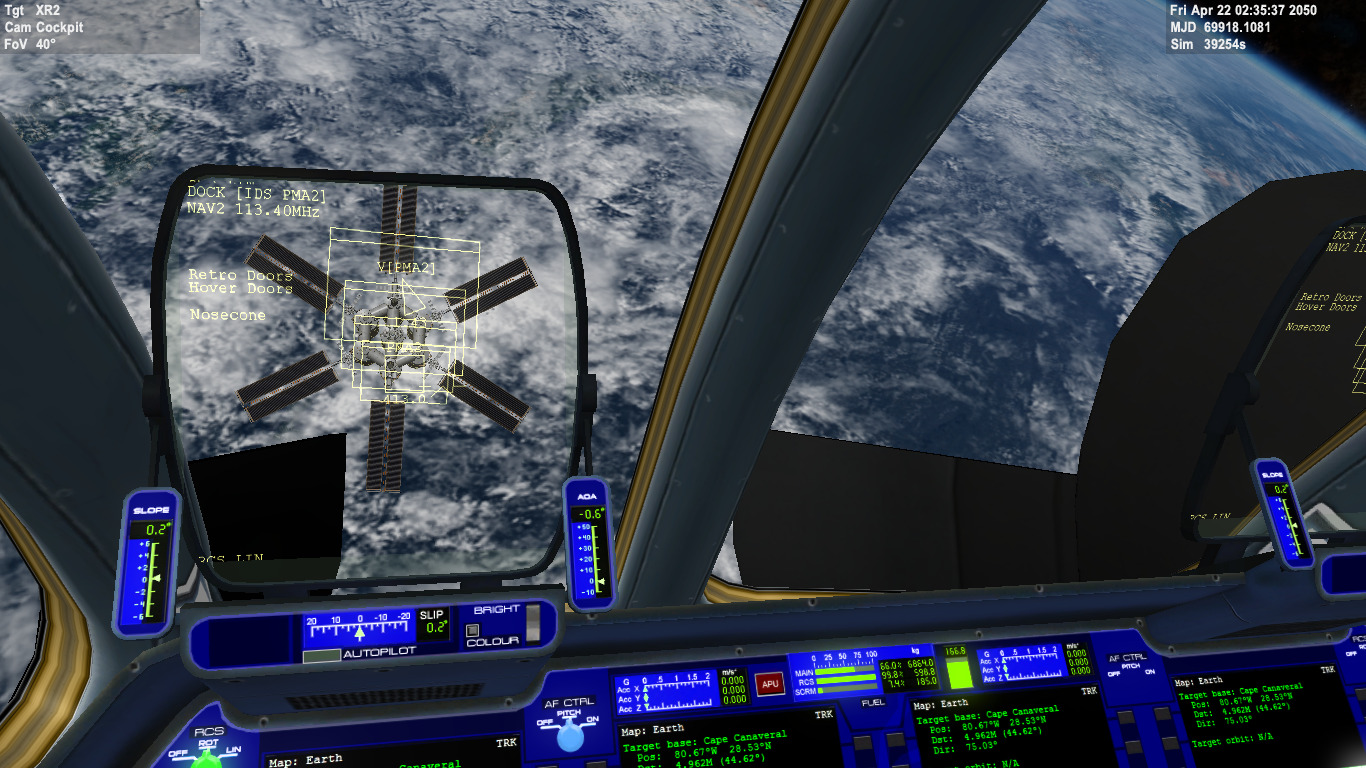
\includegraphics[width=\textwidth]{orbiter}\\
      \href{https://openorbiter.space/}{Open Orbiter Sim}\\
      former Orbiter 2016, open source since 2021, realistic, many mods
    \end{center}
  \end{minipage}
  \begin{minipage}[t]{0.49\textwidth}
    \begin{center}
      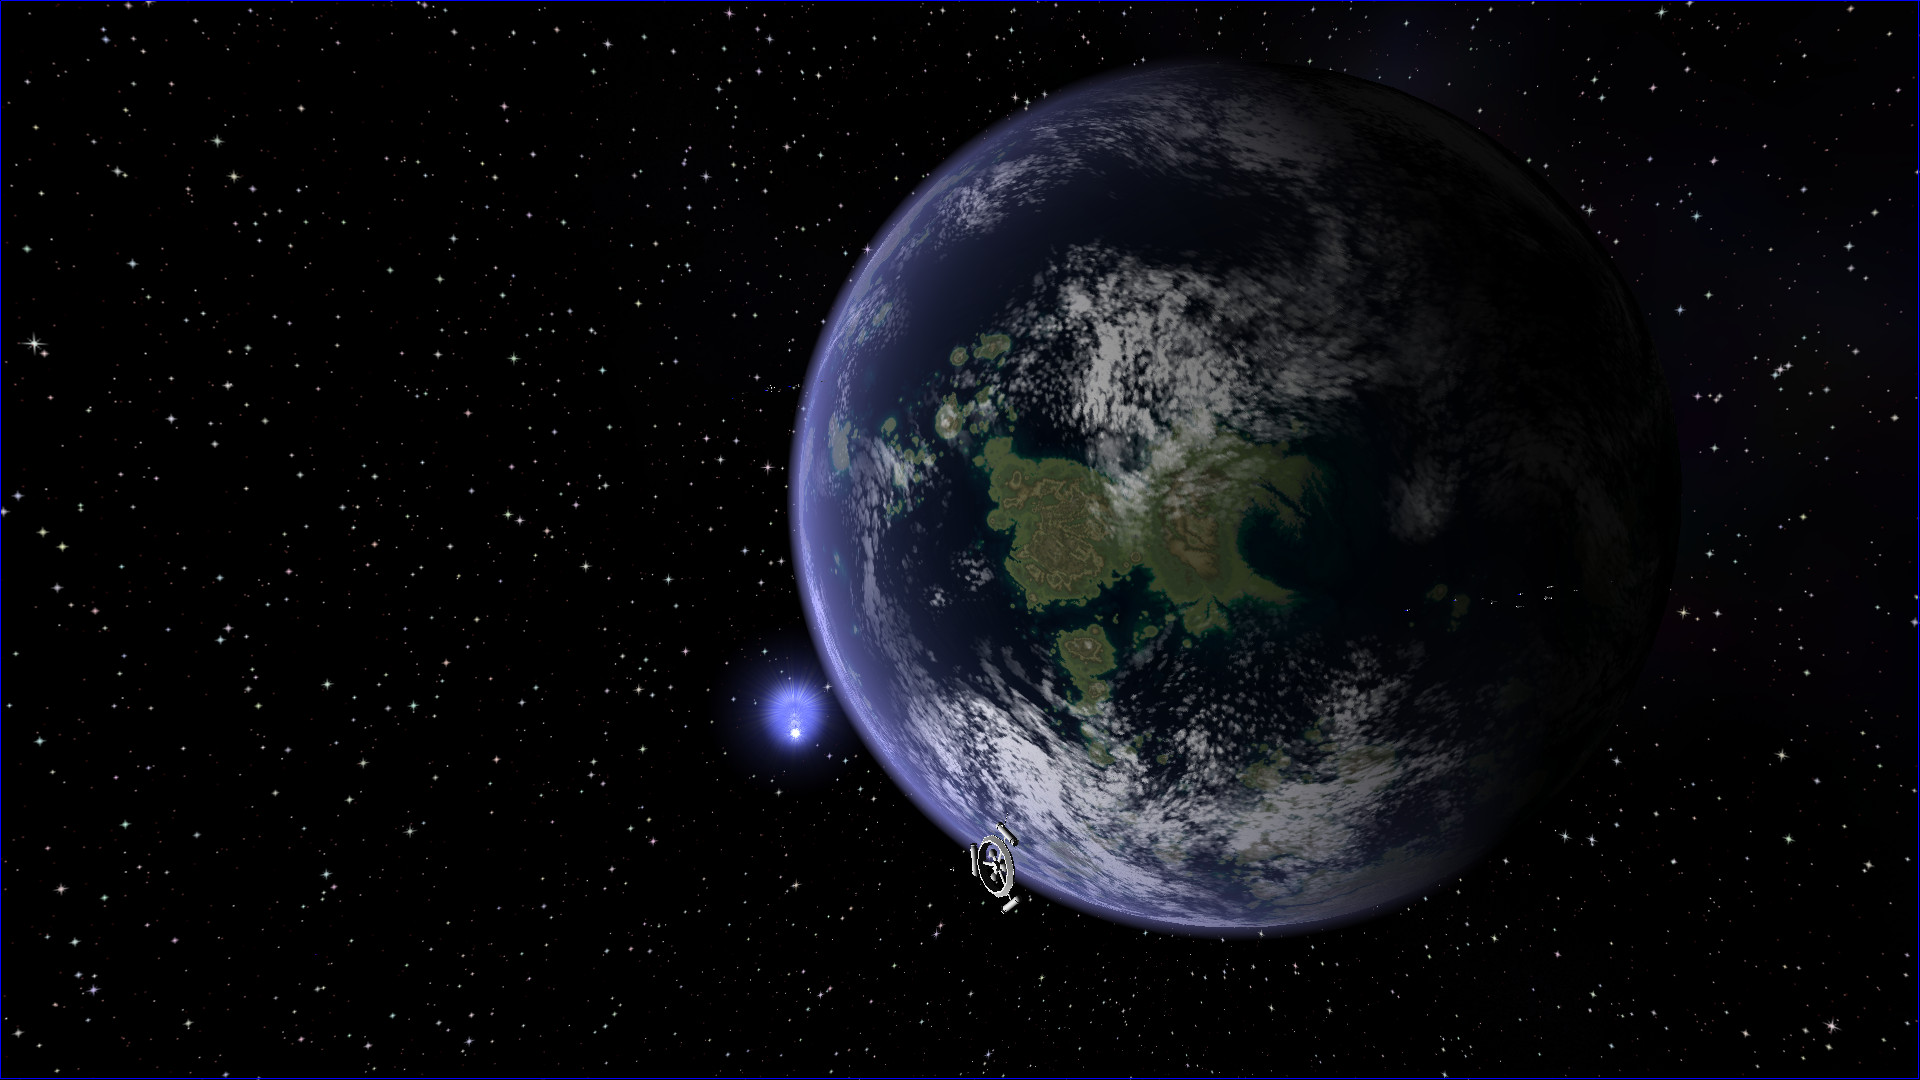
\includegraphics[width=\textwidth]{nerds}\\
      \href{https://smcameron.github.io/space-nerds-in-space/}{Space Nerds in Space}\\
      multiplayer star ship bridge sim, open source
    \end{center}
  \end{minipage}
\end{frame}

\begin{frame}
  \frametitle{Space Flight Simulator Examples 2/4}
  \begin{minipage}[t]{0.49\textwidth}
    \begin{center}
      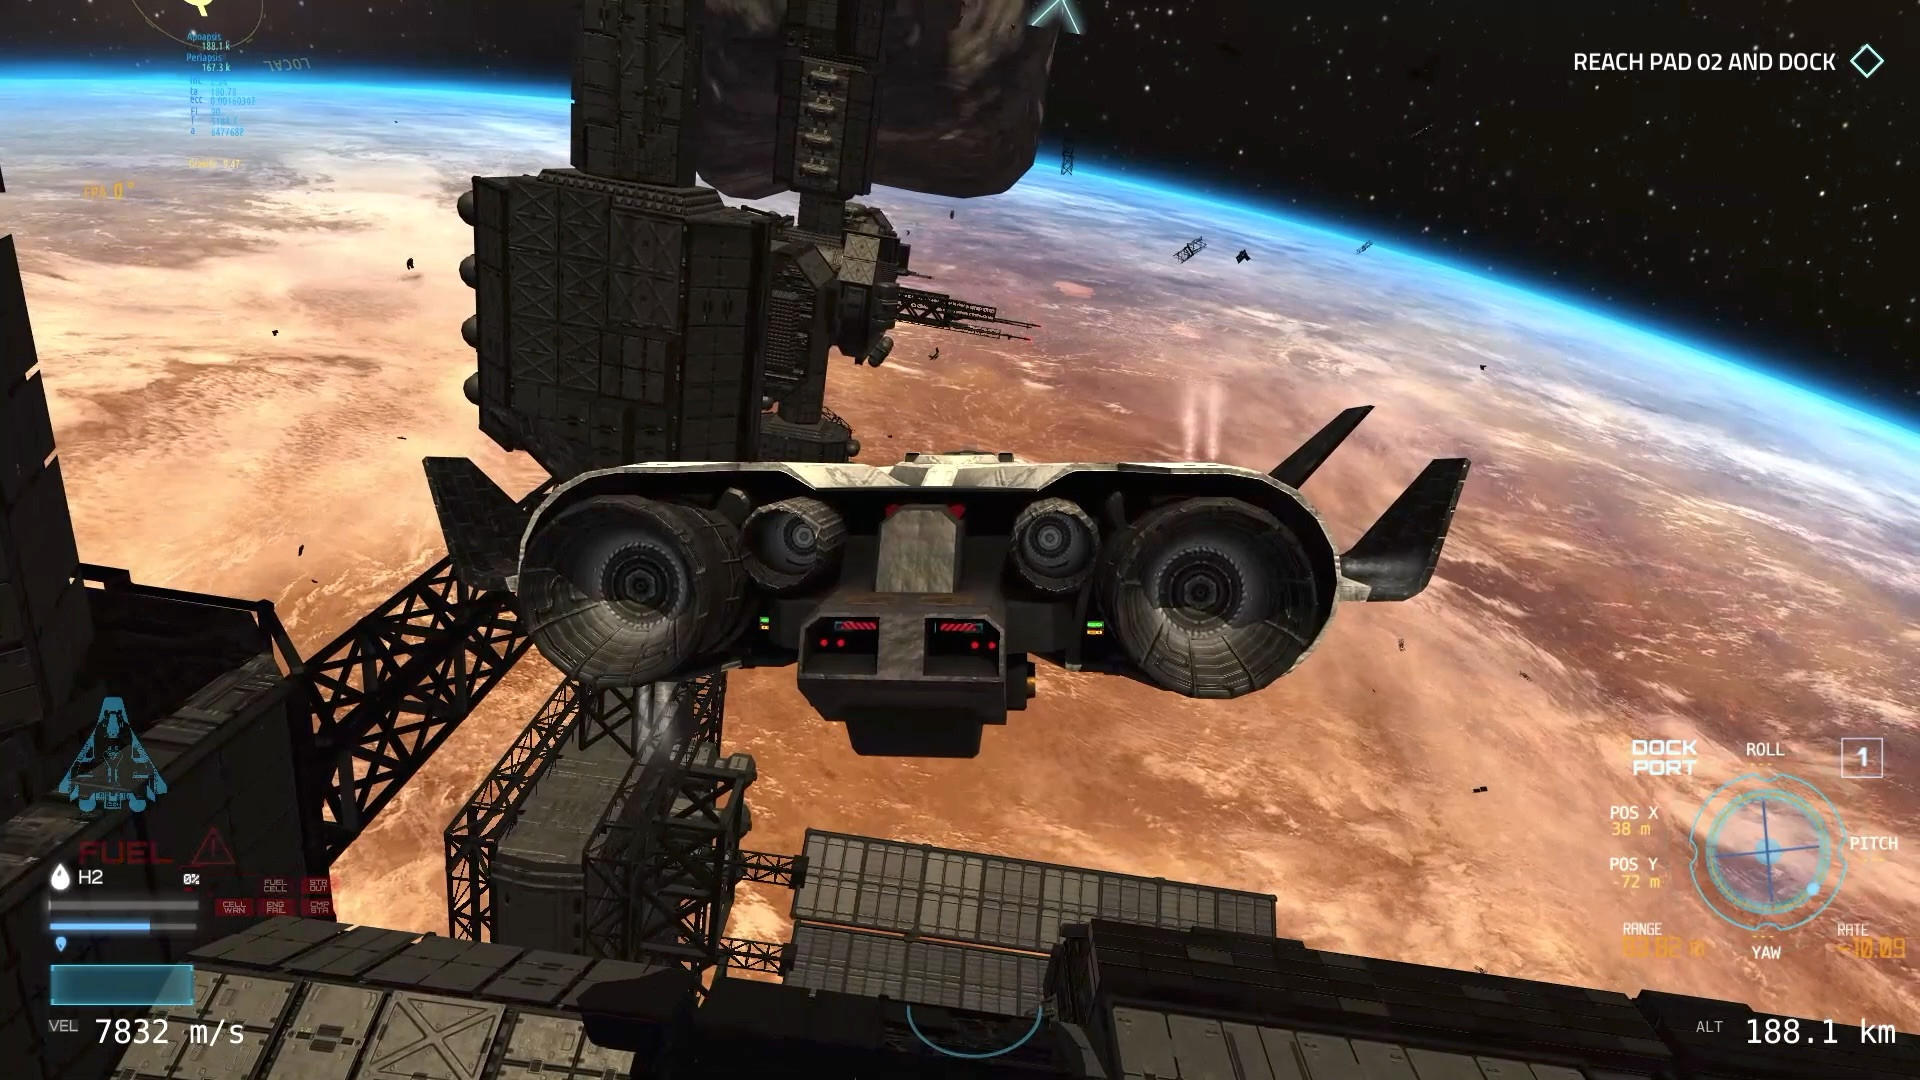
\includegraphics[width=\textwidth]{flight-of-nova}\\
      \href{https://flight-of-nova.com/}{Flight of Nova}\\
      realistic, early access
    \end{center}
  \end{minipage}
  \begin{minipage}[t]{0.49\textwidth}
    \begin{center}
      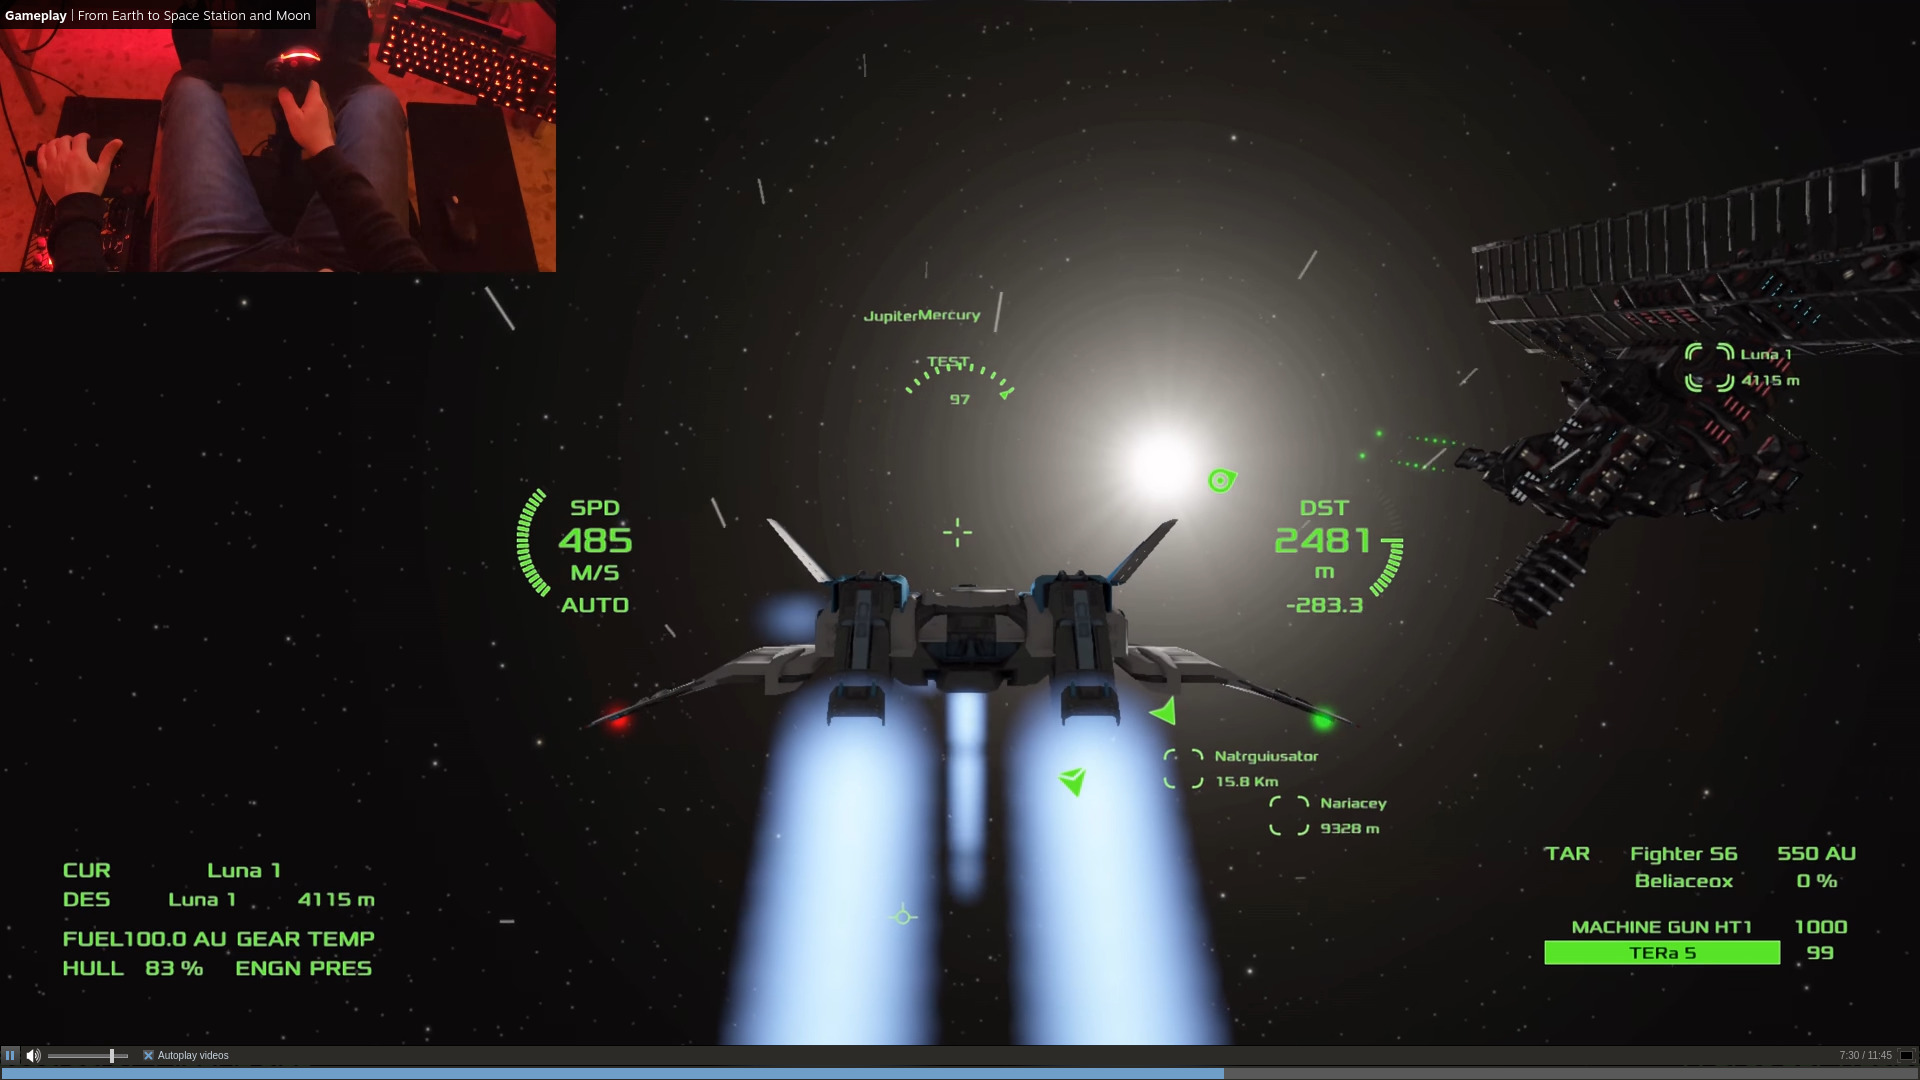
\includegraphics[width=\textwidth]{univoyager}\\
      \href{https://www.univoyager.com/}{Univoyager}\\
      real terrain with procedural detail, to be released
    \end{center}
  \end{minipage}
\end{frame}

\begin{frame}
  \frametitle{Space Flight Simulator Examples 3/4}
  \begin{minipage}[t]{0.49\textwidth}
    \begin{center}
      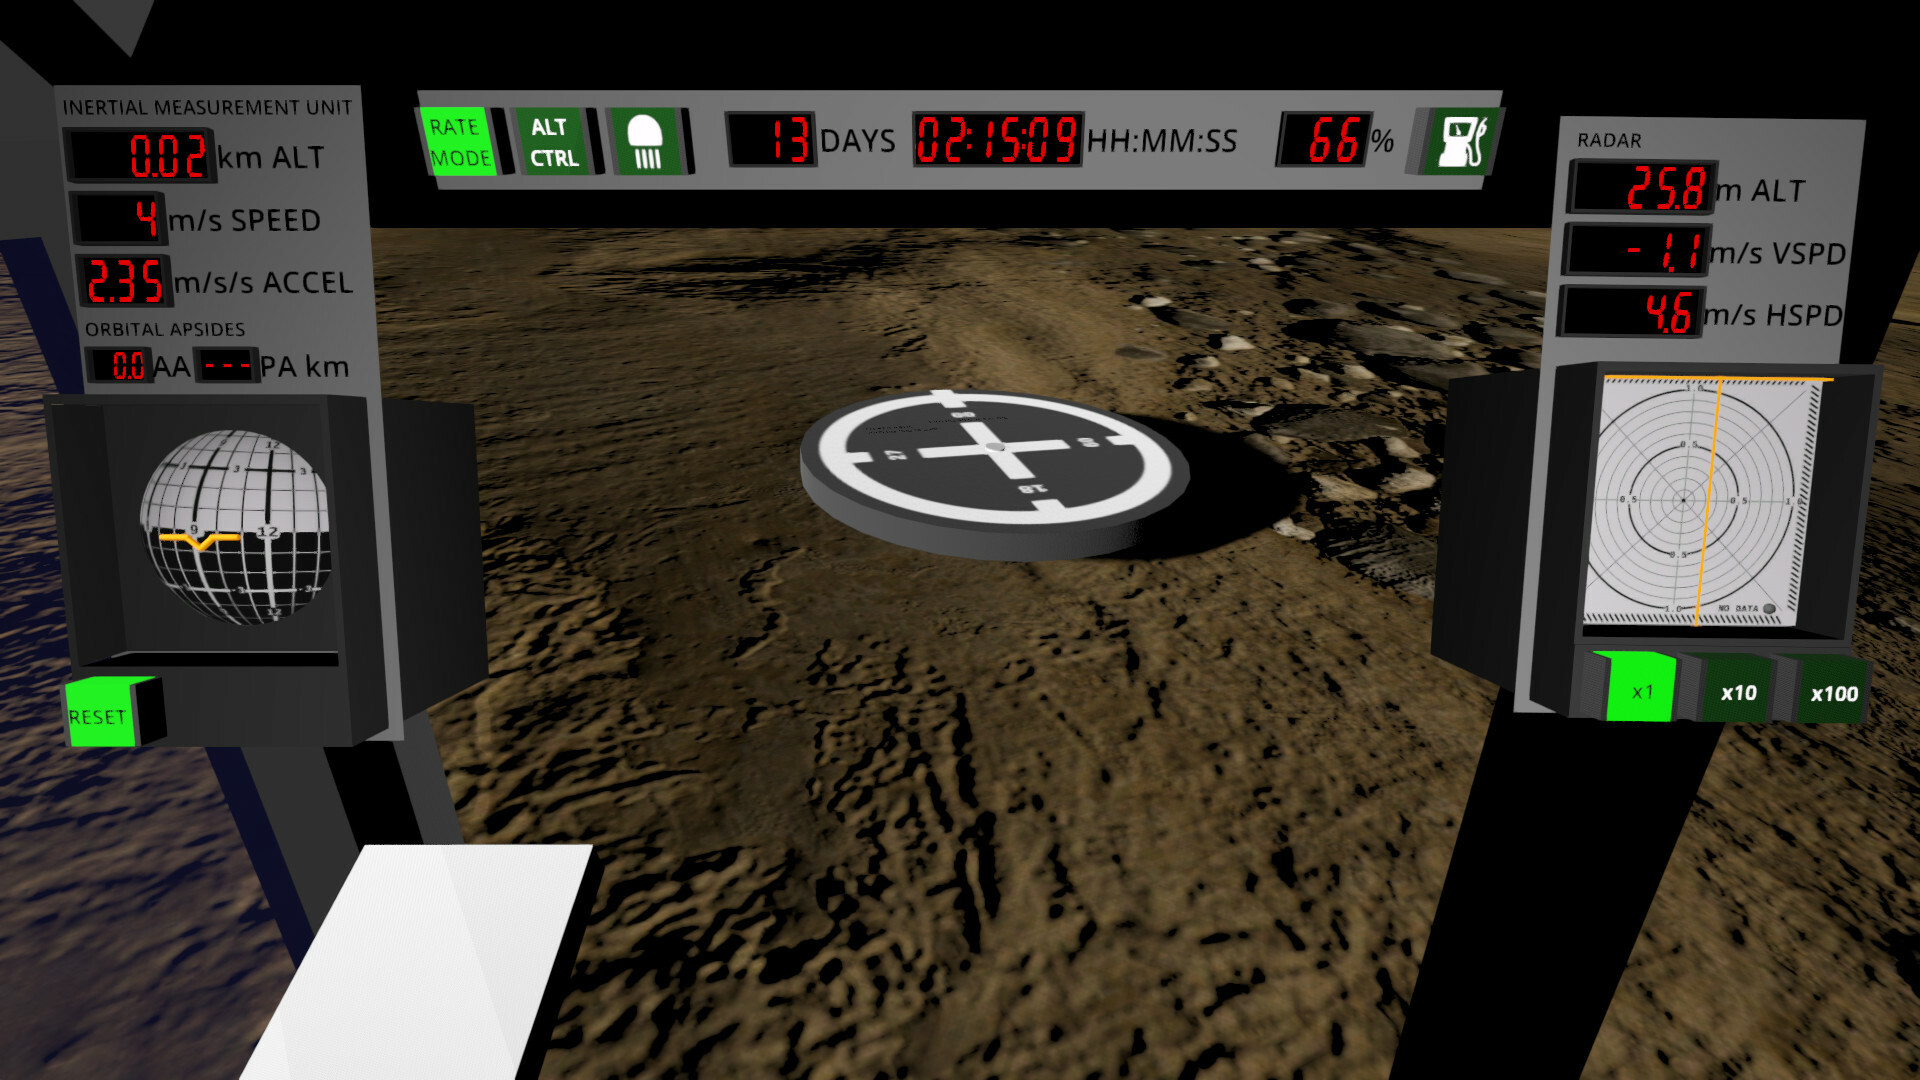
\includegraphics[width=\textwidth]{tungsten-moon}\\
      \href{https://tungstenmoon.com/}{Tungsten Moon}\\
      realistic, to be released
    \end{center}
  \end{minipage}
  \begin{minipage}[t]{0.49\textwidth}
    \begin{center}
      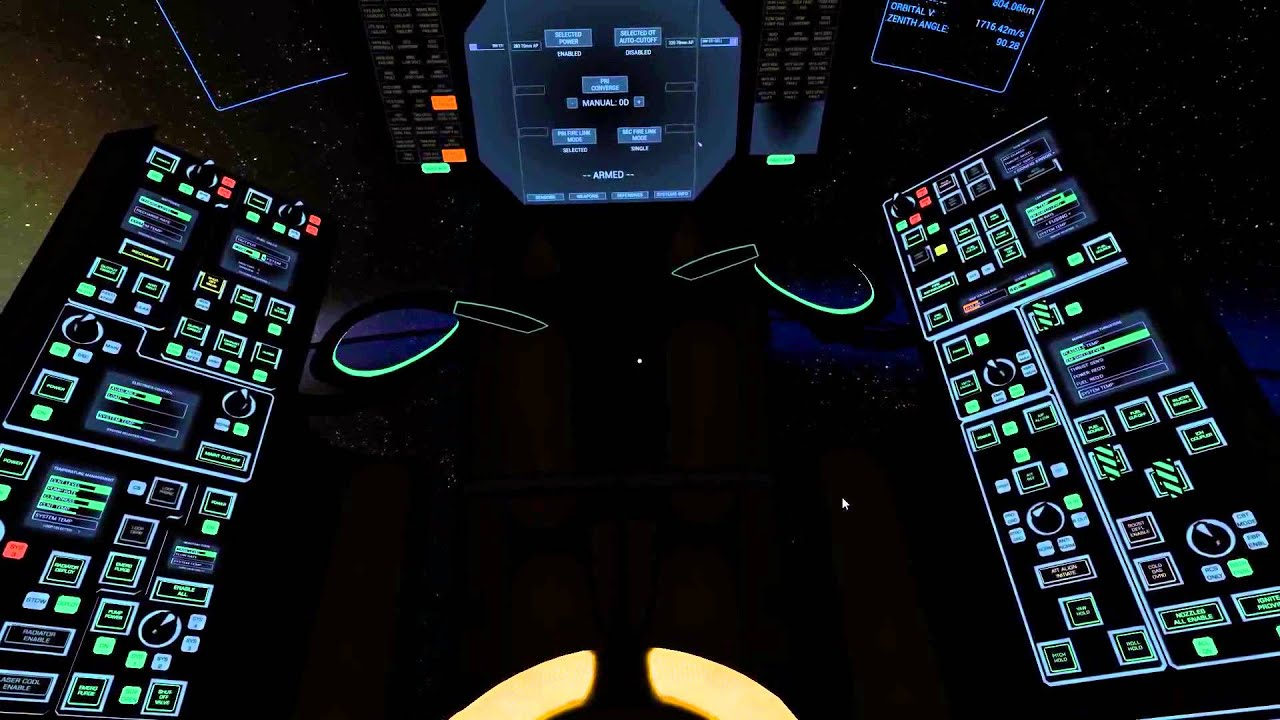
\includegraphics[width=\textwidth]{rogue-system}\\
      \href{https://imagespaceinc.com/rogsys/}{Rogue System}\\
      detailed cockpit, development on hold
    \end{center}
  \end{minipage}
\end{frame}

\begin{frame}
  \frametitle{Space Flight Simulator Examples 4/4}
  \begin{minipage}[t]{0.49\textwidth}
    \begin{center}
      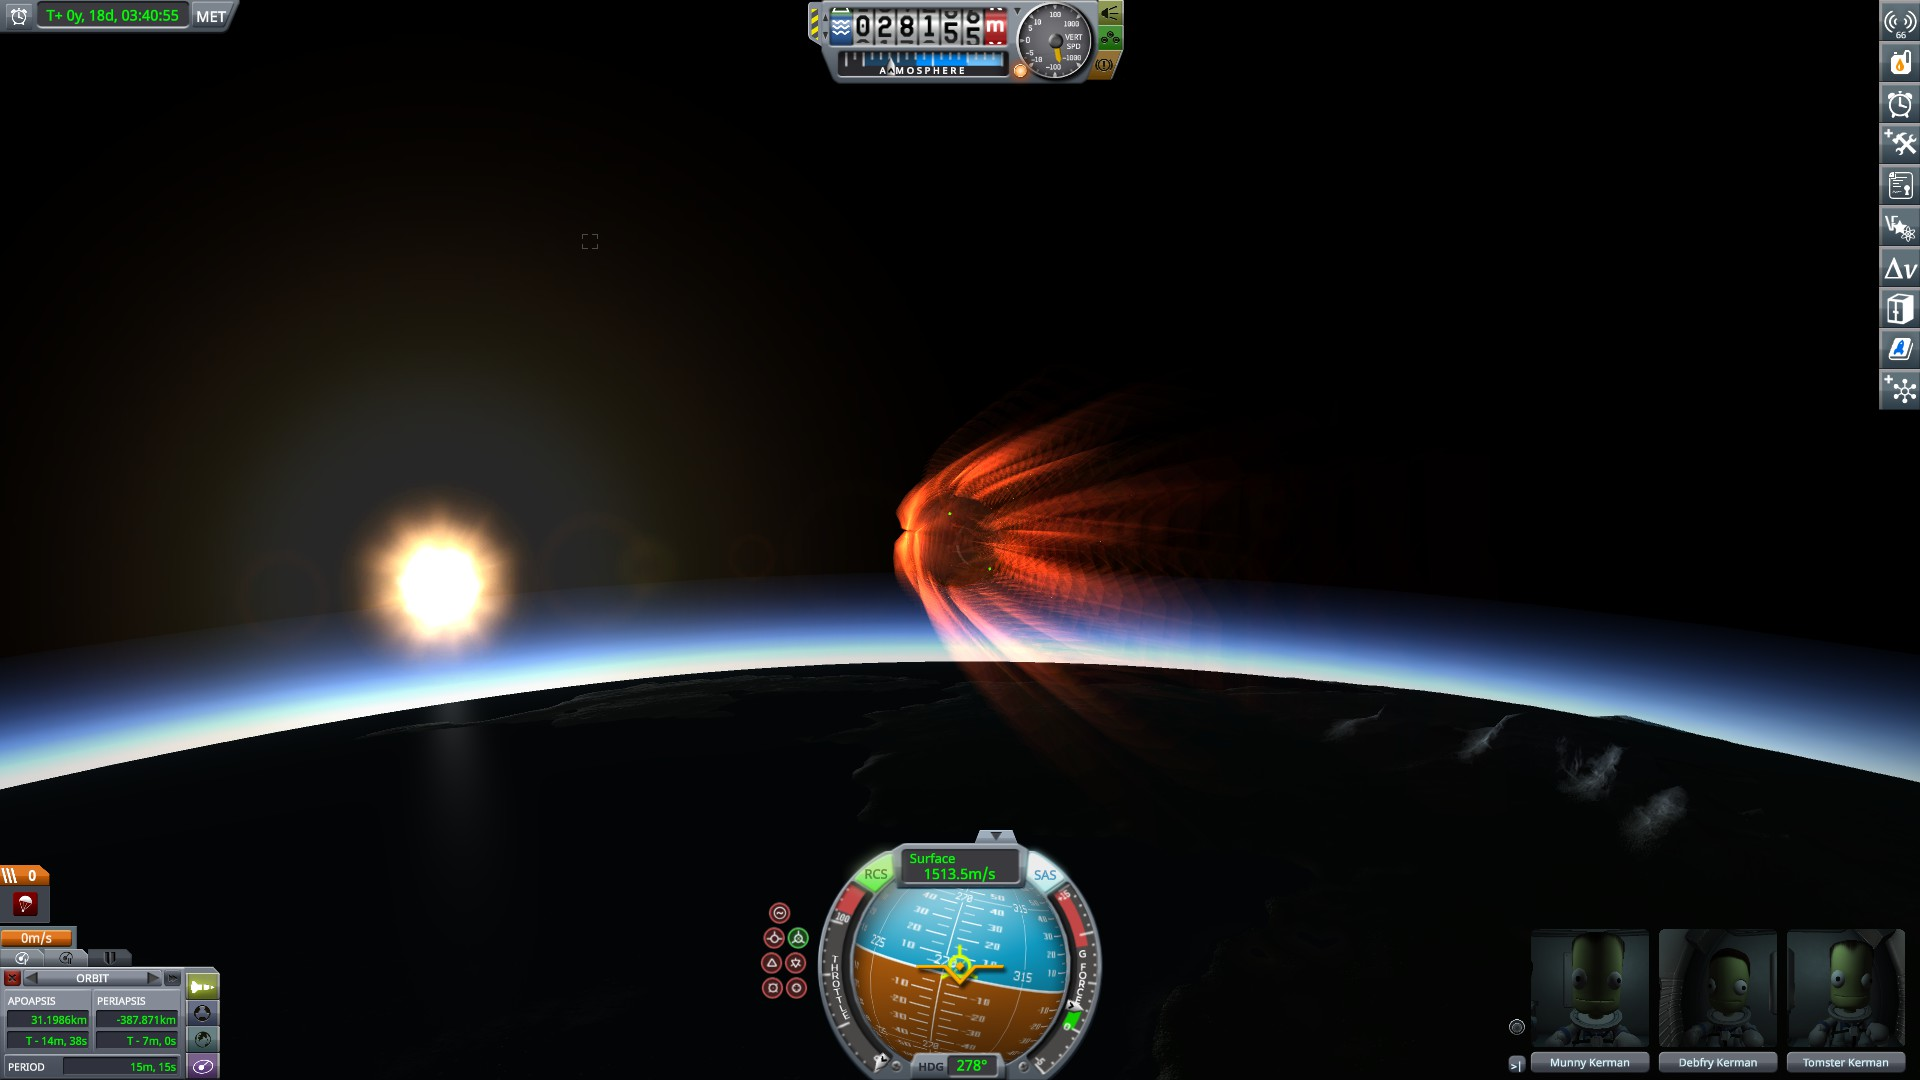
\includegraphics[width=\textwidth]{ksp}\\
      \href{https://www.kerbalspaceprogram.com/}{Kerbal Space Program}\\
      proprietary, realistic, small scale planets, many mods, KSP 2 team disbanded
    \end{center}
  \end{minipage}
  \begin{minipage}[t]{0.49\textwidth}
    \begin{center}
      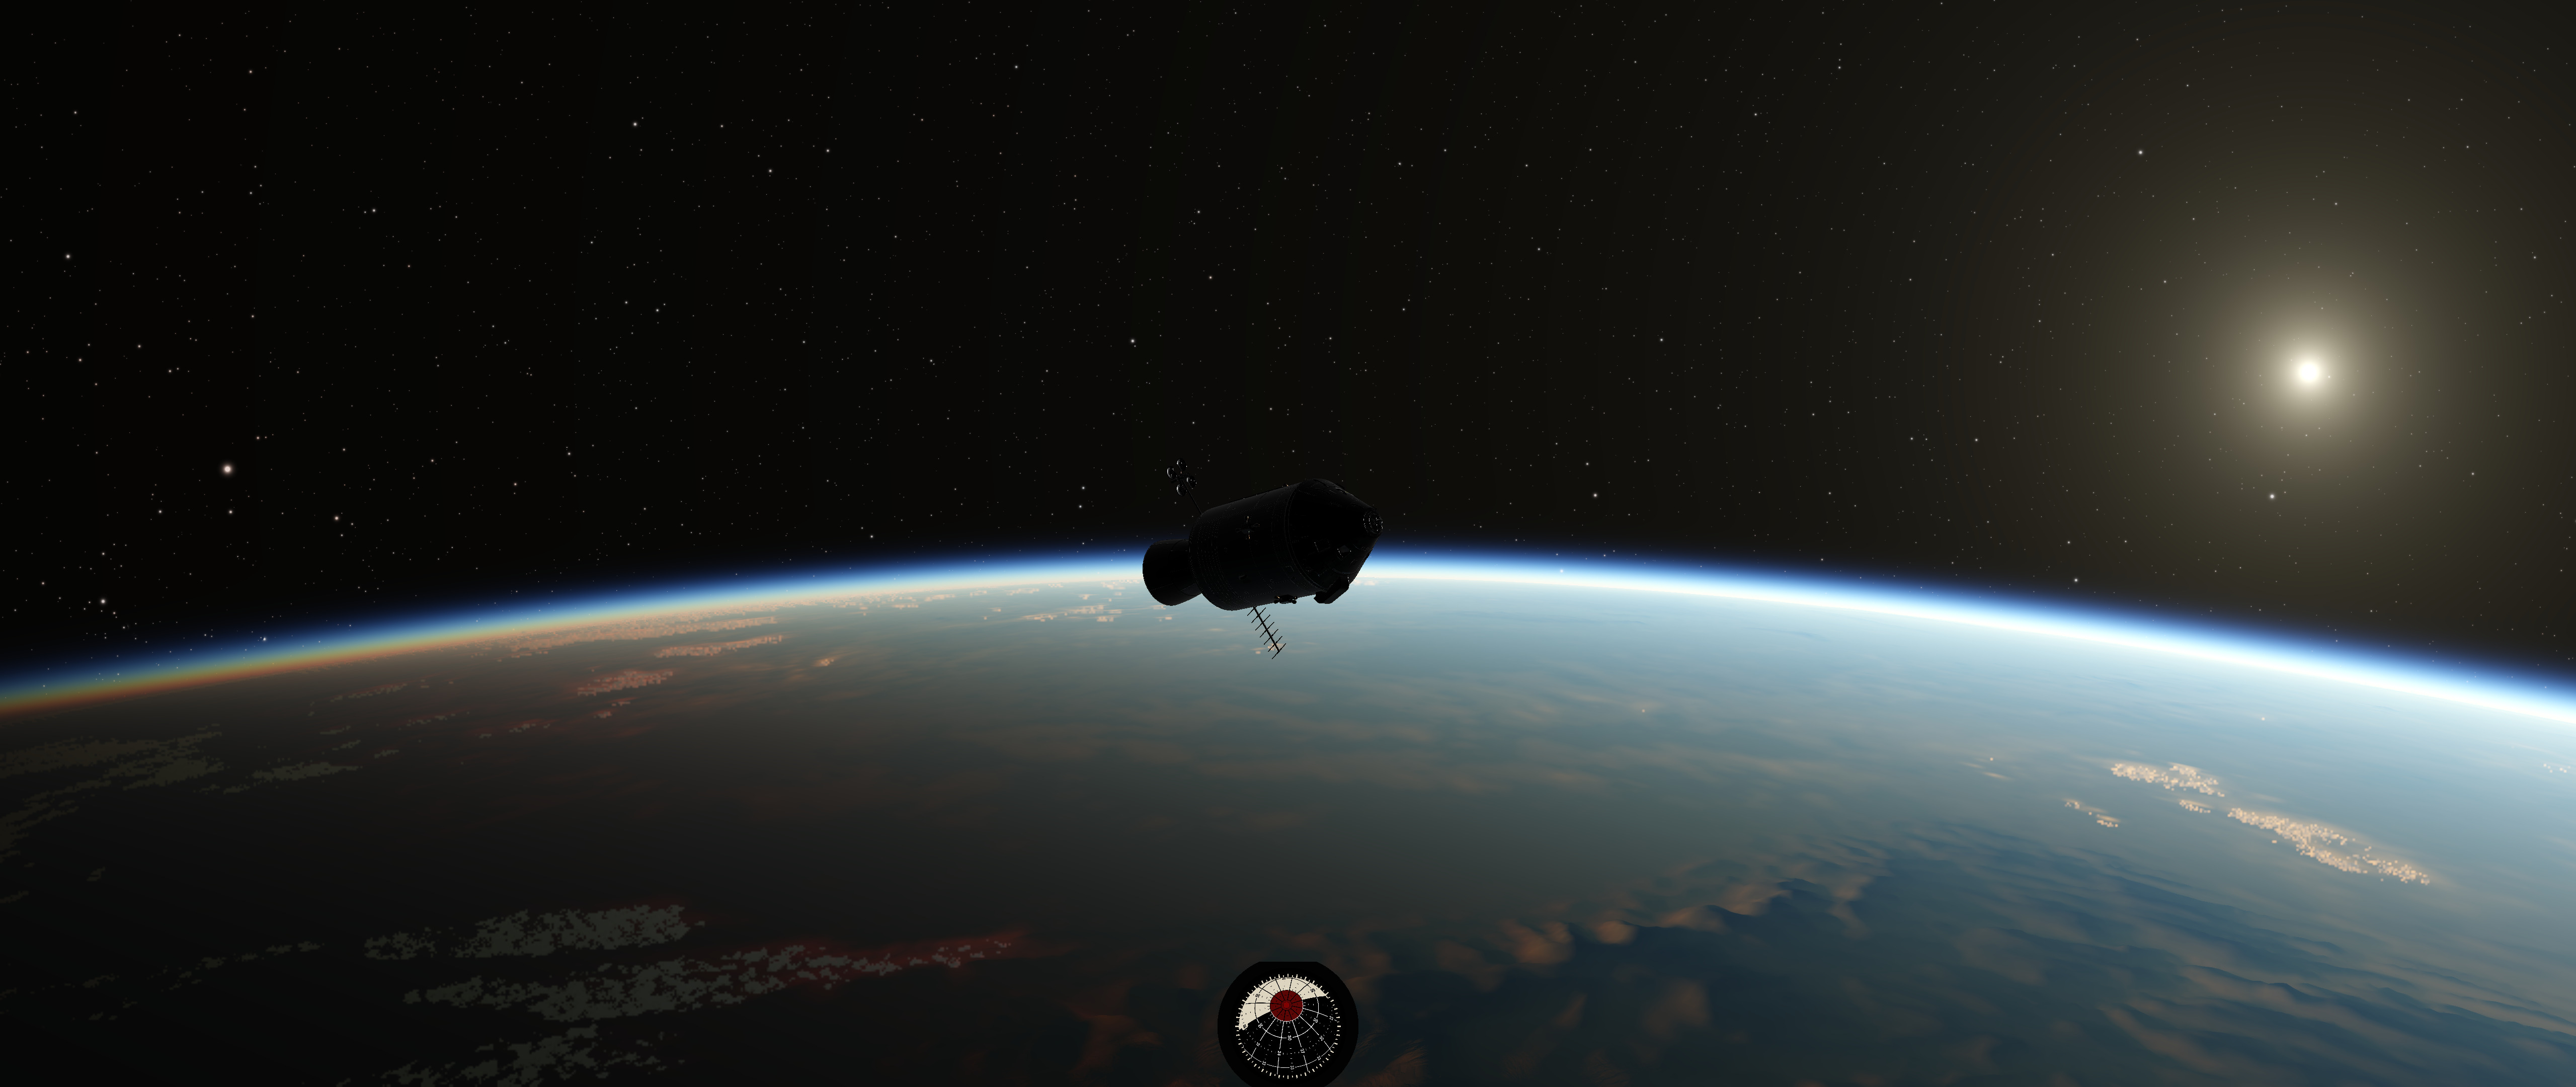
\includegraphics[width=\textwidth]{ksa}\\
      \href{https://rocketwerkz.com/}{Kitten Space Agency}\\
      proprietary, realistic, spiritual successor to KSP 2
    \end{center}
  \end{minipage}
\end{frame}

\begin{frame}
  \pdfbookmark[1]{OpenGL Superbible}{superbible}
  \frametitle{OpenGL Superbible}
  \begin{center}
    
\includegraphics[width=.35\textwidth]{superbible}\\
    \url{https://tinyurl.com/superbible}
  \end{center}
\end{frame}

\begin{frame}[fragile]
  \pdfbookmark[1]{Dependencies}{plainwindowdeps}
  \pdfbookmark[2]{deps.edn}{depsedn}
  \frametitle{deps.edn}
  \begin{minted}[]{clj}
;; Replace linux with windows or macos as appropriate:
{:deps {org.clojure/clojure {:mvn/version "1.12.2"}
        generateme/fastmath {:mvn/version "2.4.0"
          :exclusions [com.github.haifengl/smile-mkl org.bytedeco/openblas]}
        org.lwjgl/lwjgl {:mvn/version "3.3.6"}
        org.lwjgl/lwjgl$natives-linux {:mvn/version "3.3.6"}
        org.lwjgl/lwjgl-opengl {:mvn/version "3.3.6"}
        org.lwjgl/lwjgl-opengl$natives-linux {:mvn/version "3.3.6"}
        org.lwjgl/lwjgl-glfw {:mvn/version "3.3.6"}
        org.lwjgl/lwjgl-glfw$natives-linux {:mvn/version "3.3.6"}
        org.lwjgl/lwjgl-stb {:mvn/version "3.3.6"}
        org.lwjgl/lwjgl-stb$natives-linux {:mvn/version "3.3.6"}}
 :paths ["."]}
  \end{minted}
\end{frame}

\begin{frame}[fragile]
  \pdfbookmark[2]{Import}{import}
  \frametitle{Importing Libraries}
  \begin{minted}[]{clj}
(require '[clojure.java.io :as io]
         '[clojure.math :refer (PI to-radians)]
         '[fastmath.vector :refer (vec3 sub add mult normalize)])
(import '[javax.imageio ImageIO]
        '[org.lwjgl BufferUtils]
        '[org.lwjgl.glfw GLFW
                         GLFWCursorPosCallbackI
                         GLFWMouseButtonCallbackI]
        '[org.lwjgl.opengl GL GL11 GL13 GL15 GL20 GL30])
  \end{minted}
\end{frame}

\begin{frame}
  \pdfbookmark[1]{Plain Window}{plainwindow}
  \frametitle{Plain Window}
  \begin{center}
    \begin{huge}
      Creating a Plain Window
    \end{huge}
  \end{center}
\end{frame}

\begin{frame}[fragile]
  \pdfbookmark[2]{Create}{plainwindowcreate}
  \frametitle{Plain Window {-} Create}
  \begin{minted}[]{clj}
;; Initialise GLFW library and create a window with OpenGL context:
(GLFW/glfwInit)

(def window-width 1280)
(def window-height 720)

(GLFW/glfwDefaultWindowHints)
(def window
     (GLFW/glfwCreateWindow window-width window-height "example" 0 0))

(GLFW/glfwShowWindow window)
(GLFW/glfwMakeContextCurrent window)
(GL/createCapabilities)
  \end{minted}
\end{frame}

\begin{frame}[fragile]
  \pdfbookmark[2]{Event Loop}{plainwindowloop}
  \frametitle{Plain Window {-} Event Loop}
  \begin{minted}[]{clj}
;; Run event loop as follows:
(while (not (GLFW/glfwWindowShouldClose window))
       (GL11/glClearColor 0.0 1.0 0.0 1.0)
       (GL11/glClear GL11/GL_COLOR_BUFFER_BIT)
       (GLFW/glfwSwapBuffers window)
       (GLFW/glfwPollEvents))
  \end{minted}
\end{frame}

\begin{frame}[fragile]
  \pdfbookmark[2]{Terminate}{plainwindowterminate}
  \frametitle{Plain Window {-} Terminate}
  \begin{minted}[]{clj}
;; Terminate the program like this:
(GLFW/glfwDestroyWindow window)
(GLFW/glfwTerminate)
  \end{minted}
\end{frame}

\begin{frame}
  \pdfbookmark[2]{Result}{plainwindowresult}
  \frametitle{Plain Window {-} Result}
  \begin{center}
    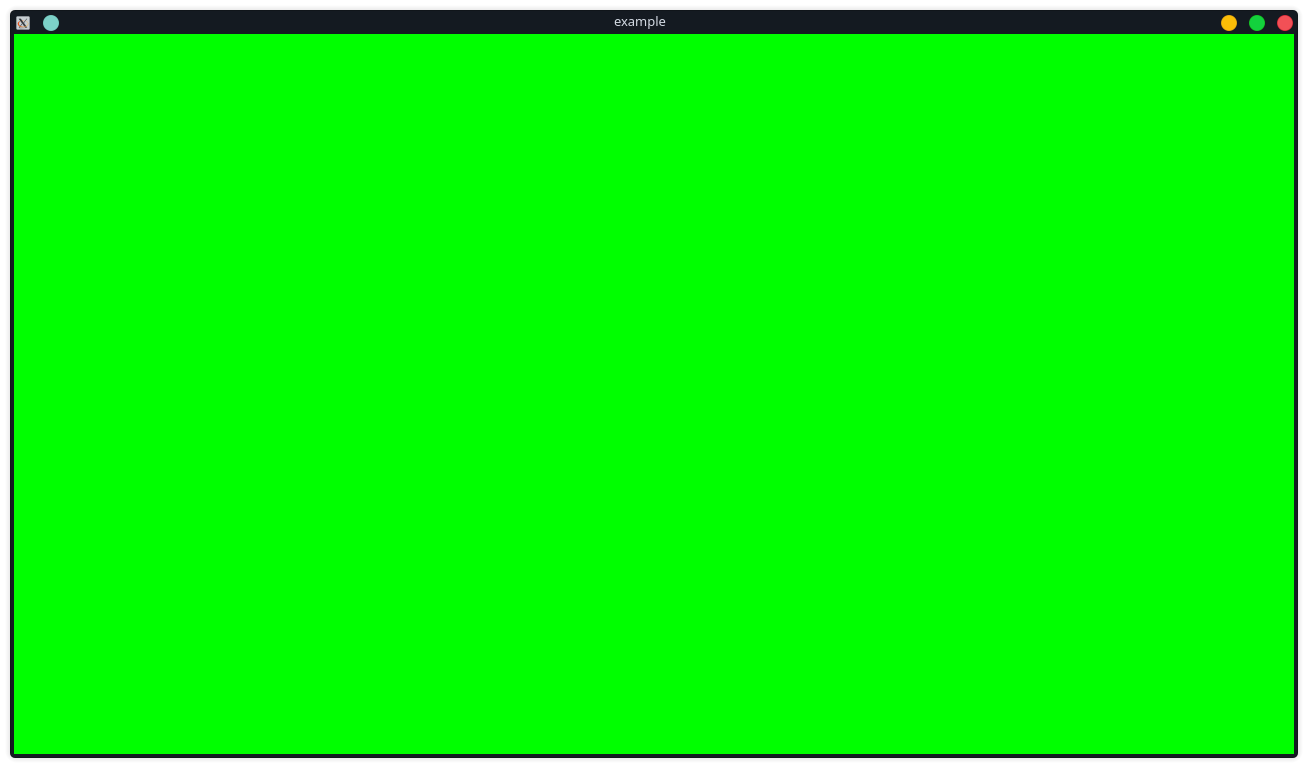
\includegraphics[width=.8\textwidth]{window}
  \end{center}
\end{frame}

\begin{frame}
  \pdfbookmark[1]{Single Quad}{quad}
  \frametitle{Single Quad}
  \begin{center}
    \begin{huge}
      Rendering a Single Quad
    \end{huge}
  \end{center}
\end{frame}

\begin{frame}[fragile]
  \pdfbookmark[2]{Vertex Shader}{quadvertex}
  \frametitle{Single Quad {-} Vertex Shader}
  \begin{minted}[]{glsl}
#version 130
in vec3 point;
void main()
{
  gl_Position = vec4(point, 1);
}
  \end{minted}
  \rule{\textwidth}{1pt}
  \begin{minted}[]{clj}
(def vertex-source "
#version 130
in vec3 point;
void main()
{
  gl_Position = vec4(point, 1);
}")
  \end{minted}
\end{frame}

\begin{frame}[fragile]
  \pdfbookmark[2]{Fragment Shader}{quadfragment}
  \frametitle{Single Quad {-} Fragment Shader}
  \begin{minted}[]{glsl}
#version 130
uniform vec2 iResolution;
out vec4 fragColor;
void main()
{
  vec2 uv = gl_FragCoord.xy / iResolution.xy;
  fragColor = vec4(uv, 0, 1);
}
  \end{minted}
  \rule{\textwidth}{1pt}
  \begin{minted}[]{clj}
(def fragment-source "
#version 130

// ...

")
  \end{minted}
\end{frame}

\begin{frame}[fragile]
  \pdfbookmark[2]{Compiling Shaders}{quadcompile}
  \frametitle{Single Quad {-} Compiling Shaders}
  \begin{minted}[]{clj}
(defn make-shader [source shader-type]
  (let [shader (GL20/glCreateShader shader-type)]
    (GL20/glShaderSource shader source)
    (GL20/glCompileShader shader)
    (when (zero? (GL20/glGetShaderi shader GL20/GL_COMPILE_STATUS))
      (throw (Exception. (GL20/glGetShaderInfoLog shader 1024))))
    shader))

(def vertex-shader (make-shader vertex-source GL20/GL_VERTEX_SHADER))
(def fragment-shader (make-shader fragment-source GL20/GL_FRAGMENT_SHADER))
  \end{minted}
\end{frame}

\begin{frame}[fragile]
  \pdfbookmark[2]{Linking Shader Program}{quadlink}
  \frametitle{Single Quad {-} Linking Shader Program}
  \begin{minted}[]{clj}
(defn make-program [& shaders]
  (let [program (GL20/glCreateProgram)]
    (doseq [shader shaders]
           (GL20/glAttachShader program shader)
           (GL20/glDeleteShader shader))
    (GL20/glLinkProgram program)
    (when (zero? (GL20/glGetProgrami program GL20/GL_LINK_STATUS))
      (throw (Exception. (GL20/glGetProgramInfoLog program 1024))))
    program))

(def program (make-program vertex-shader fragment-shader))
  \end{minted}
\end{frame}

\begin{frame}[fragile]
  \pdfbookmark[2]{Vertices and Indices}{quadvertices}
  \frametitle{Single Quad {-} Vertices and Indices}
  \begin{minted}[]{clj}
(def vertices  ;   x    y   z
  (float-array [ 1.0  1.0 0.0,
                -1.0  1.0 0.0,
                -1.0 -1.0 0.0,
                 1.0 -1.0 0.0]))

(def indices
  (int-array [0 1 2 3]))
  \end{minted}
\end{frame}

\begin{frame}[fragile]
  \pdfbookmark[2]{Buffers}{quadbuffers}
  \frametitle{Single Quad {-} Buffers}
  \begin{minted}[]{clj}
(defmacro def-make-buffer [method create-buffer]
  `(defn ~method [data#]
     (let [buffer# (~create-buffer (count data#))]
       (.put buffer# data#)
       (.flip buffer#)
       buffer#)))

(def-make-buffer make-float-buffer BufferUtils/createFloatBuffer)
(def-make-buffer make-int-buffer BufferUtils/createIntBuffer)
(def-make-buffer make-byte-buffer BufferUtils/createByteBuffer)
  \end{minted}
\end{frame}

\begin{frame}[fragile]
  \pdfbookmark[2]{Vertex Array Object}{quadvao}
  \frametitle{Single Quad {-} Vertex Array Object}
  \begin{minted}[]{clj}
(defn setup-vao [vertices indices]
  (let [vao (GL30/glGenVertexArrays)
        vbo (GL15/glGenBuffers)
        ibo (GL15/glGenBuffers)]
    (GL30/glBindVertexArray vao)
    (GL15/glBindBuffer GL15/GL_ARRAY_BUFFER vbo)
    (GL15/glBufferData GL15/GL_ARRAY_BUFFER
                       (make-float-buffer vertices) GL15/GL_STATIC_DRAW)
    (GL15/glBindBuffer GL15/GL_ELEMENT_ARRAY_BUFFER ibo)
    (GL15/glBufferData GL15/GL_ELEMENT_ARRAY_BUFFER
                       (make-int-buffer indices) GL15/GL_STATIC_DRAW)
    {:vao vao :vbo vbo :ibo ibo}))

(def vao (setup-vao vertices indices))
  \end{minted}
\end{frame}

\begin{frame}[fragile]
  \pdfbookmark[2]{Vertex Attributes Layout}{quadattributes}
  \frametitle{Single Quad {-} Vertex Attributes Layout}
  \begin{minted}[]{clj}
(def point (GL20/glGetAttribLocation program "point"))
; void glVertexAttribPointer(index, size, type, normalized,
;                            stride, pointer);
(GL20/glVertexAttribPointer point 3 GL11/GL_FLOAT false
                            (* 3 Float/BYTES) (* 0 Float/BYTES))
(GL20/glEnableVertexAttribArray point)
  \end{minted}
\end{frame}

\begin{frame}[fragile]
  \pdfbookmark[2]{Uniform Variables}{quaduniforms}
  \frametitle{Single Quad {-} Uniform Variables}
  \begin{minted}[]{clj}
(GL20/glUseProgram program)
(GL20/glUniform2f (GL20/glGetUniformLocation program "iResolution")
                  window-width window-height)
  \end{minted}
\end{frame}

\begin{frame}[fragile]
  \pdfbookmark[2]{Event Loop}{quadloop}
  \frametitle{Single Quad {-} Event Loop}
  \begin{minted}[]{clj}
(while (not (GLFW/glfwWindowShouldClose window))
       (GL11/glClearColor 0.0 0.0 0.0 1.0)
       (GL11/glClear GL11/GL_COLOR_BUFFER_BIT)
       (GL11/glDrawElements GL11/GL_QUADS (count indices)
                            GL11/GL_UNSIGNED_INT 0)
       (GLFW/glfwSwapBuffers window)
       (GLFW/glfwPollEvents))
  \end{minted}
\end{frame}

\begin{frame}[fragile]
  \pdfbookmark[2]{Terminate}{quadterminate}
  \frametitle{Single Quad {-} Terminate}
  \begin{minted}[]{clj}
(defn teardown-vao [{:keys [vao vbo ibo]}]
  (GL15/glBindBuffer GL15/GL_ELEMENT_ARRAY_BUFFER 0)
  (GL15/glDeleteBuffers ibo)
  (GL15/glBindBuffer GL15/GL_ARRAY_BUFFER 0)
  (GL15/glDeleteBuffers vbo)
  (GL30/glBindVertexArray 0)
  (GL15/glDeleteBuffers vao))

(teardown-vao vao)

(GL20/glDeleteProgram program)
  \end{minted}
\end{frame}

\begin{frame}
  \pdfbookmark[2]{Result}{quadresult}
  \frametitle{Single Quad {-} Result}
  \begin{center}
    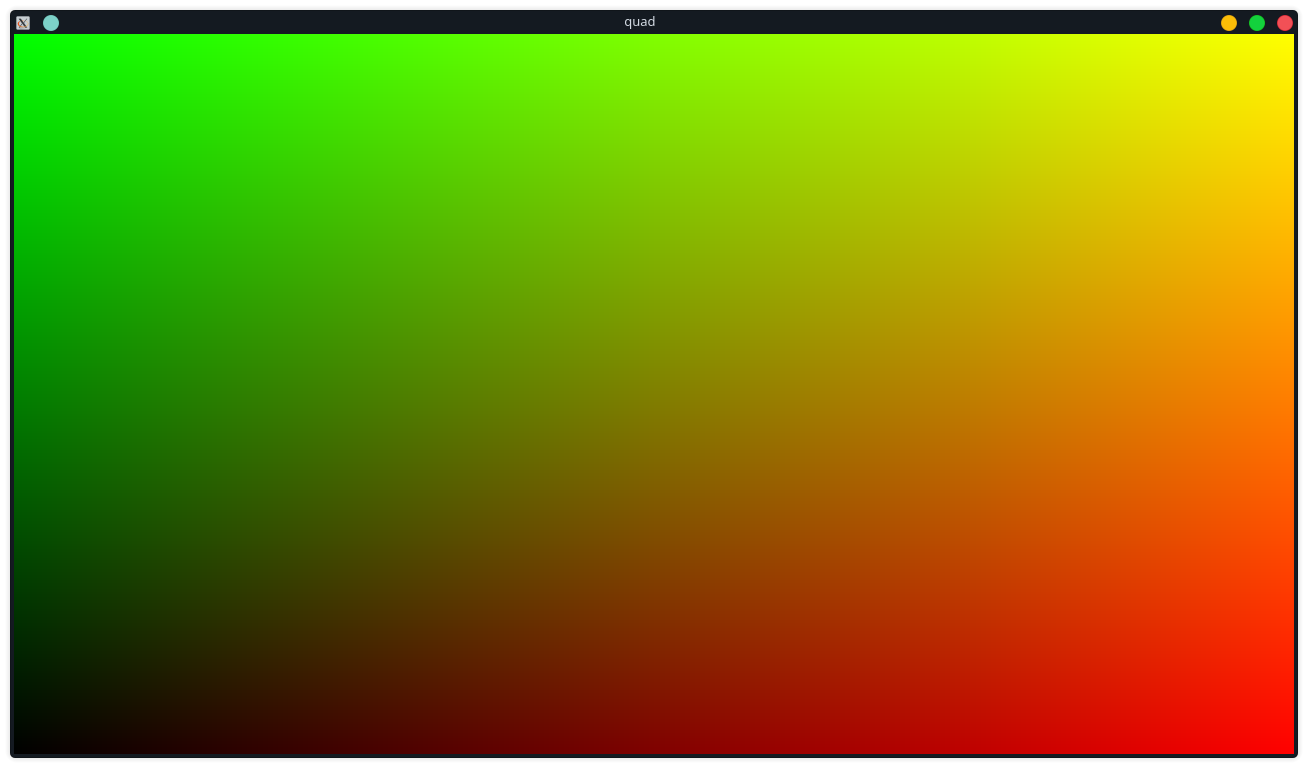
\includegraphics[width=.8\textwidth]{quad}
  \end{center}
\end{frame}

\begin{frame}
  \pdfbookmark[1]{Texture}{texture}
  \frametitle{Texture}
  \begin{center}
    \begin{huge}
      Rendering a Texture
    \end{huge}
  \end{center}
\end{frame}

\begin{frame}[fragile]
  \pdfbookmark[2]{Load Image}{textureload}
  \frametitle{Texture {-} Load Image}
  \begin{minted}[]{clj}
(def color (ImageIO/read (io/file "lroc_color_poles_2k.tif")))
(def color-raster (.getRaster color))
(def color-width (.getWidth color-raster))
(def color-height (.getHeight color-raster))
(def color-channels (.getNumBands color-raster))
(def color-pixels (int-array (* color-width color-height color-channels)))
(.getPixels color-raster 0 0 color-width color-height color-pixels)
  \end{minted}
\end{frame}

\begin{frame}[fragile]
  \pdfbookmark[2]{Create Texture}{texturecreate}
  \frametitle{Texture {-} Create Texture}
  \begin{minted}[]{clj}
(def buffer (make-byte-buffer (byte-array (map unchecked-byte color-pixels))))
(def texture-color (GL11/glGenTextures))
(GL11/glBindTexture GL11/GL_TEXTURE_2D texture-color)
(GL11/glTexImage2D GL11/GL_TEXTURE_2D 0 GL11/GL_RGBA
                   color-width color-height 0
                   GL11/GL_RGB GL11/GL_UNSIGNED_BYTE
                   buffer)
(GL11/glTexParameteri GL11/GL_TEXTURE_2D GL11/GL_TEXTURE_MIN_FILTER
                      GL11/GL_LINEAR)
(GL11/glTexParameteri GL11/GL_TEXTURE_2D GL11/GL_TEXTURE_MAG_FILTER
                      GL11/GL_LINEAR)
(GL11/glTexParameteri GL11/GL_TEXTURE_2D GL11/GL_TEXTURE_WRAP_S
                      GL11/GL_REPEAT)
(GL11/glTexParameteri GL11/GL_TEXTURE_2D GL11/GL_TEXTURE_WRAP_T
                      GL11/GL_REPEAT)
(GL11/glBindTexture GL11/GL_TEXTURE_2D 0)
  \end{minted}
\end{frame}

\begin{frame}[fragile]
  \pdfbookmark[2]{Color Lookup}{texturecolor}
  \frametitle{Texture {-} Color Lookup}
  \begin{minted}[]{glsl}
#version 130

uniform sampler2D moon;

vec3 color(vec2 uv)
{
  return texture(moon, uv).rgb;
}
  \end{minted}
\end{frame}

\begin{frame}[fragile]
  \pdfbookmark[2]{Fragment Shader}{texturefragment}
  \frametitle{Texture {-} Fragment Shader}
  \begin{minted}[]{glsl}
#version 130

uniform vec2 iResolution;
out vec4 fragColor;

vec3 color(vec2 uv);

void main()
{
  fragColor = vec4(color(gl_FragCoord.xy / iResolution.xy), 1.0);
}
  \end{minted}
\end{frame}

\begin{frame}[fragile]
  \pdfbookmark[2]{Uniform Variables}{textureuniforms}
  \frametitle{Texture {-} Uniform Variables}
  \begin{minted}[]{clj}
(GL20/glUniform1i (GL20/glGetUniformLocation program "moon") 0)
(GL13/glActiveTexture GL13/GL_TEXTURE0)
(GL11/glBindTexture GL11/GL_TEXTURE_2D texture-color)
  \end{minted}
\end{frame}

\begin{frame}[fragile]
  \pdfbookmark[2]{Terminate}{textureterminate}
  \frametitle{Texture {-} Terminate}
  \begin{minted}[]{clj}
(GL11/glDeleteTextures texture-color)
  \end{minted}
\end{frame}

\begin{frame}
  \pdfbookmark[2]{Result}{textureresult}
  \frametitle{Texture {-} Result}
  \begin{center}
    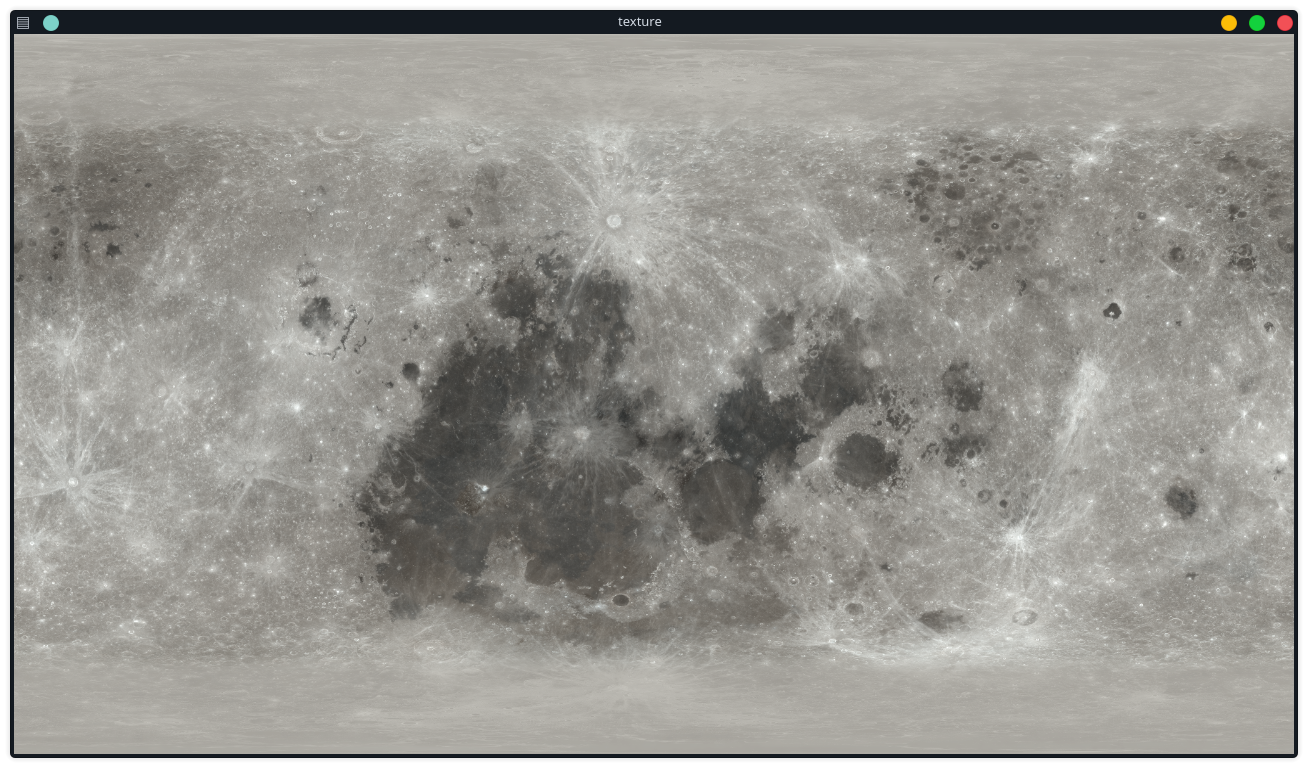
\includegraphics[width=.8\textwidth]{texture}
  \end{center}
\end{frame}

\begin{frame}
  \pdfbookmark[1]{Cube}{cube}
  \frametitle{Cube}
  \begin{center}
    \begin{huge}
      Rendering a Cube
    \end{huge}
  \end{center}
\end{frame}

\begin{frame}[fragile]
  \pdfbookmark[2]{Mouse Callbacks}{cubemouse}
  \frametitle{Cube {-} Mouse Callbacks}
  \begin{minted}[]{clj}
(def mouse-pos (atom [0.0 0.0]))
(def mouse-button (atom false))

(GLFW/glfwSetCursorPosCallback
  window
  (reify GLFWCursorPosCallbackI
    (invoke
      [_this _window xpos ypos]
      (reset! mouse-pos [xpos ypos]))))

(GLFW/glfwSetMouseButtonCallback
  window
  (reify GLFWMouseButtonCallbackI
    (invoke
      [_this _window _button action _mods]
      (reset! mouse-button (= action GLFW/GLFW_PRESS)))))
  \end{minted}
\end{frame}

\begin{frame}[fragile]
  \pdfbookmark[2]{Vertex Shader}{cubevertex}
  \frametitle{Cube {-} Vertex Shader 1/2}
  \begin{minted}[]{glsl}
#version 130
#define M_PI 3.1415926535897932384626433832795
uniform float fov;
uniform float distance;
uniform vec2 iResolution;
uniform vec2 iMouse;
in vec3 point;
out vec3 vpoint;
void main()
{
  float alpha = iMouse.x / iResolution.x * M_PI * 2.0 + M_PI;
  float beta = (iMouse.y / iResolution.y - 0.5) * M_PI * 2.0;
  // ...
}
  \end{minted}
\end{frame}

\begin{frame}[fragile]
  \frametitle{Cube {-} Vertex Shader 2/2}
  \begin{minted}[]{glsl}
{ // ...
  mat3 rot_y = mat3(vec3(cos(alpha), 0, sin(alpha)),
                    vec3(0, 1, 0),
                    vec3(-sin(alpha), 0, cos(alpha)));
  mat3 rot_x = mat3(vec3(1, 0, 0),
                    vec3(0, cos(beta), -sin(beta)),
                    vec3(0, sin(beta), cos(beta)));
  vec3 p = rot_x * rot_y * point + vec3(0, 0, distance);
  float f = 1.0 / tan(fov / 2.0);
  float aspect = iResolution.x / iResolution.y;
  float proj_x = p.x / p.z * f;
  float proj_y = p.y / p.z * f * aspect;
  float proj_z = p.z / (2.0 * distance);
  gl_Position = vec4(proj_x, proj_y, proj_z, 1);
  vpoint = point;
}
  \end{minted}
\end{frame}

\begin{frame}[fragile]
  \pdfbookmark[2]{Map Texture onto Sphere}{cubemap}
  \frametitle{Cube {-} Map Texture onto Sphere}
  \begin{minted}[]{glsl}
#version 130

#define PI 3.1415926535897932384626433832795

vec2 uv(vec3 p)
{
  float u = atan(p.x, -p.z) / (2.0 * PI) + 0.5;
  float v = 0.5 - atan(p.y, length(p.xz)) / PI;
  return vec2(u, v);
}
  \end{minted}
\end{frame}

\begin{frame}[fragile]
  \pdfbookmark[2]{Fragment Shader}{cubefragment}
  \frametitle{Cube {-} Fragment Shader}
  \begin{minted}[]{glsl}
#version 130

in vec3 vpoint;
out vec4 fragColor;

vec2 uv(vec3 p);
vec3 color(vec2 uv);

void main()
{
  fragColor = vec4(color(uv(vpoint)), 1);
}
  \end{minted}
\end{frame}

\begin{frame}[fragile]
  \pdfbookmark[2]{Vertices and Indices}{cubevertices}
  \frametitle{Cube {-} Vertices and Indices}
  \begin{minipage}[t]{.48\textwidth}
    \begin{minted}[]{clj}
(def vertices  ;   x    y   z
  (float-array [-1.0 -1.0 -1.0,
                 1.0 -1.0 -1.0,
                -1.0  1.0 -1.0,
                 1.0  1.0 -1.0,
                -1.0 -1.0  1.0,
                 1.0 -1.0  1.0,
                -1.0  1.0  1.0,
                 1.0  1.0  1.0]))
    \end{minted}
  \end{minipage}
  \begin{minipage}[t]{.48\textwidth}
    \begin{minted}[]{clj}
(def indices
  (int-array [0 1 3 2,
              6 7 5 4,
              0 2 6 4,
              5 7 3 1,
              2 3 7 6,
              4 5 1 0]))
    \end{minted}
  \end{minipage}
\end{frame}

\begin{frame}[fragile]
  \pdfbookmark[2]{Uniform Variables}{cubeuniforms}
  \frametitle{Cube {-} Uniform Variables}
  \begin{minted}[]{clj}
(GL20/glUniform1f (GL20/glGetUniformLocation program "fov")
                  (to-radians 35.0))
(GL20/glUniform1f (GL20/glGetUniformLocation program "distance") 10.0)
  \end{minted}
\end{frame}

\begin{frame}[fragile]
  \pdfbookmark[2]{Event Loop}{cubeloop}
  \frametitle{Cube {-} Event Loop}
  \begin{minted}[]{clj}
(GL11/glEnable GL11/GL_CULL_FACE)
(GL11/glCullFace GL11/GL_BACK)

(while (not (GLFW/glfwWindowShouldClose window))
       (when @mouse-button
         (GL20/glUniform2f (GL20/glGetUniformLocation program "iMouse")
                           (@mouse-pos 0) (@mouse-pos 1)))
       (GL11/glClearColor 0.0 0.0 0.0 1.0)
       (GL11/glClear GL11/GL_COLOR_BUFFER_BIT)
       (GL11/glDrawElements GL11/GL_QUADS (count indices)
                            GL11/GL_UNSIGNED_INT 0)
       (GLFW/glfwSwapBuffers window)
       (GLFW/glfwPollEvents))
  \end{minted}
\end{frame}

\begin{frame}
  \pdfbookmark[2]{Result}{cuberesult}
  \frametitle{Cube {-} Result}
  \begin{center}
    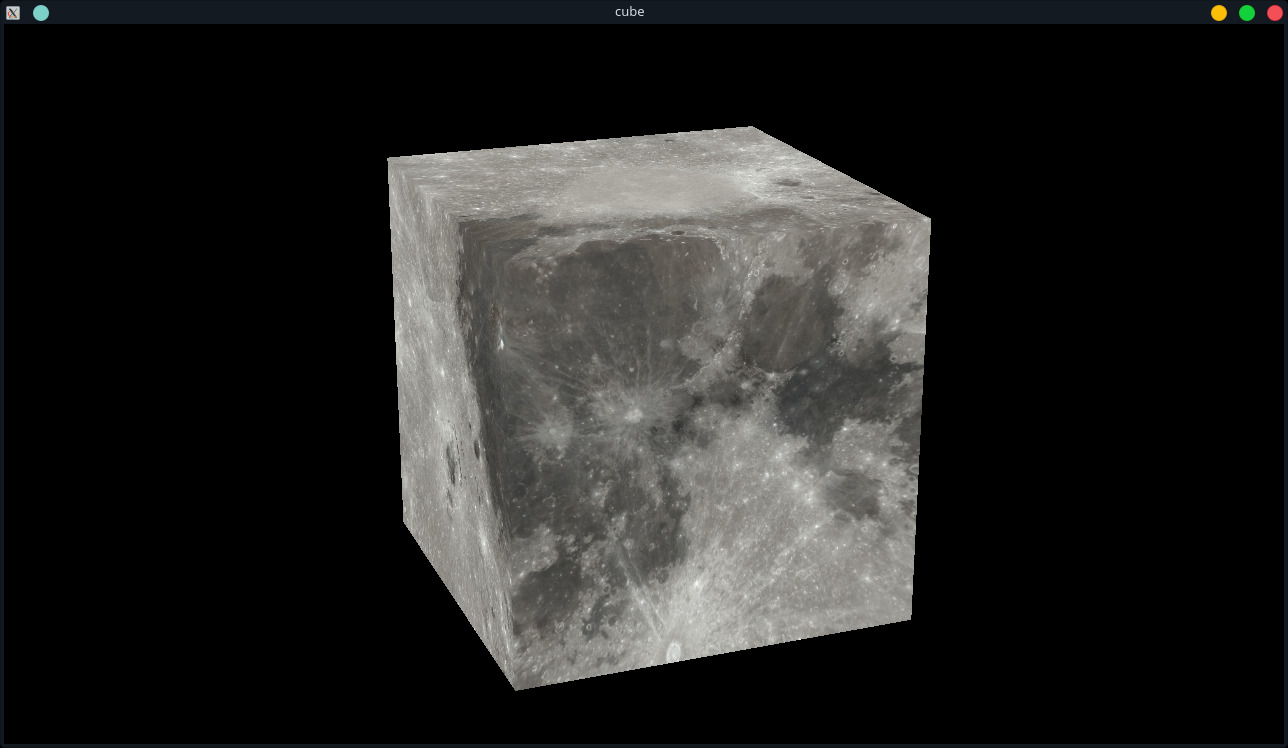
\includegraphics[width=.8\textwidth]{cube}
  \end{center}
\end{frame}

\begin{frame}
  \pdfbookmark[1]{Sphere}{sphere}
  \frametitle{Sphere}
  \begin{center}
    \begin{huge}
      Rendering a Sphere
    \end{huge}
  \end{center}
\end{frame}

\begin{frame}[fragile]
  \pdfbookmark[2]{Vertices and Indices}{spherevertices}
  \frametitle{Sphere {-} Vertices and Indices 1/4}
  \begin{minipage}[t]{.48\textwidth}
    \begin{minted}[]{clj}
(def points
  [(vec3 -1.0 -1.0 -1.0)
   (vec3  1.0 -1.0 -1.0)
   (vec3 -1.0  1.0 -1.0)
   (vec3  1.0  1.0 -1.0)
   (vec3 -1.0 -1.0  1.0)
   (vec3  1.0 -1.0  1.0)
   (vec3 -1.0  1.0  1.0)
   (vec3  1.0  1.0  1.0)])
    \end{minted}
  \end{minipage}
  \begin{minipage}[t]{.48\textwidth}
    \begin{minted}[]{clj}
(def quads
  [[0 1 3 2]
   [6 7 5 4]
   [0 2 6 4]
   [5 7 3 1]
   [2 3 7 6]
   [4 5 1 0]])
    \end{minted}
  \end{minipage}
\end{frame}

\begin{frame}[fragile]
  \frametitle{Sphere {-} Vertices and Indices 2/4}
  \begin{minted}[]{clj}
(def radius 1737.4)

(def corners
  (map (fn [[i _ _ _]] (nth points i))
       quads))

(def u-vectors
  (map (fn [[i j _ _]] (sub (nth points j) (nth points i)))
       quads))

(def v-vectors
  (map (fn [[i _ _ l]] (sub (nth points l) (nth points i)))
       quads))
  \end{minted}
\end{frame}

\begin{frame}[fragile]
  \frametitle{Sphere {-} Vertices and Indices 3/4}
  \begin{minted}[]{clj}
(defn sphere-points [n c u v]
  (for [j (range (inc n)) i (range (inc n))]
       (-> c
           (add (mult u (/ i n)))
           (add (mult v (/ j n)))
           normalize
           (mult radius ))))

(defn sphere-indices [n face]
  (for [j (range n) i (range n)]
       (let [offset (+ (* face (inc n) (inc n)) (* j (inc n)) i)]
         [offset
          (+ offset 1)
          (+ offset (inc n) 1)
          (+ offset (inc n))])))
  \end{minted}
\end{frame}

\begin{frame}[fragile]
  \frametitle{Sphere {-} Vertices and Indices 4/4}
  \begin{minted}[]{clj}
(def n 16)

(def vertices
  (float-array
    (flatten
      (map (partial sphere-points n)
           corners u-vectors v-vectors))))

(def indices
  (int-array
    (flatten
      (map (partial sphere-indices n)
           (range 6)))))
  \end{minted}
\end{frame}

\begin{frame}[fragile]
  \pdfbookmark[2]{Uniform Variables}{sphereuniforms}
  \frametitle{Sphere {-} Uniform Variables}
  \begin{minted}[]{clj}
(GL20/glUniform1f (GL20/glGetUniformLocation program "distance")
                  (* radius 10.0))
  \end{minted}
\end{frame}

\begin{frame}
  \pdfbookmark[2]{Result}{sphereresult}
  \frametitle{Sphere {-} Result}
  \begin{center}
    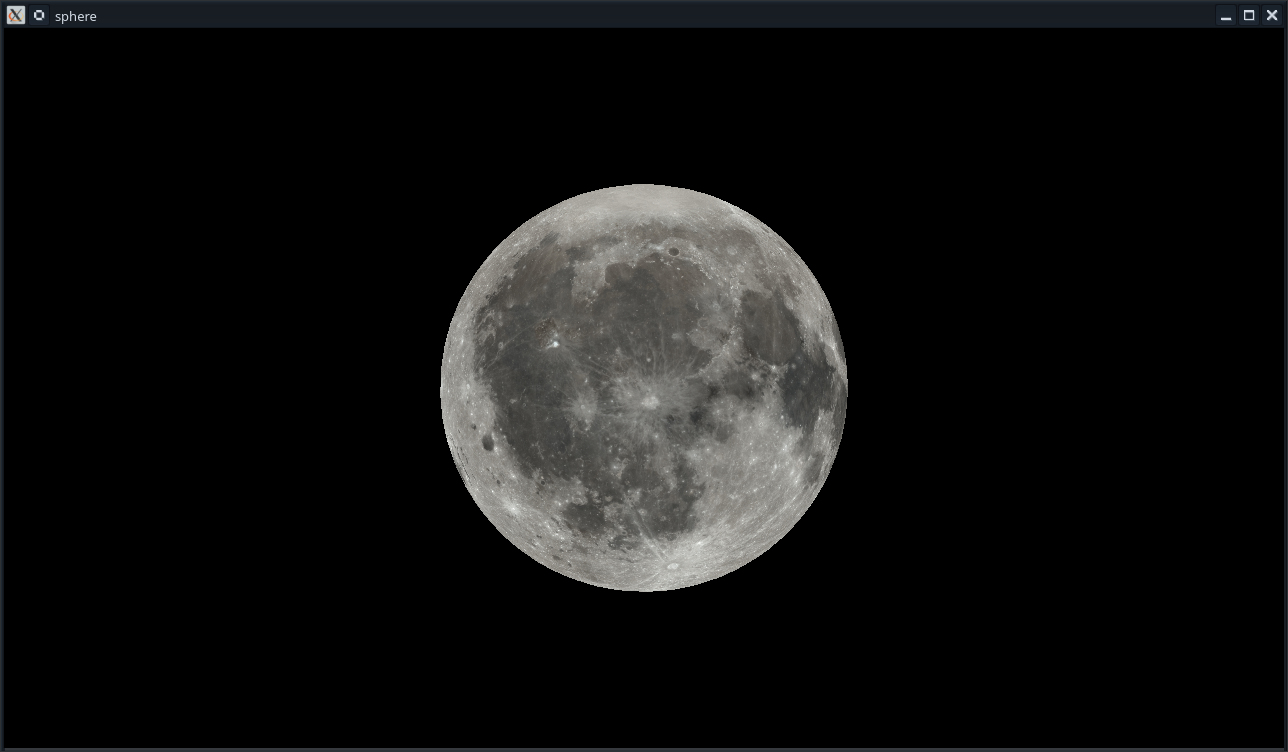
\includegraphics[width=.8\textwidth]{sphere}
  \end{center}
\end{frame}

\begin{frame}
  \pdfbookmark[1]{Moon}{moon}
  \frametitle{Moon}
  \begin{center}
    \begin{huge}
      Rendering the Moon
    \end{huge}
  \end{center}
\end{frame}

\begin{frame}[fragile]
  \pdfbookmark[2]{Load Elevation Data}{elevationload}
  \frametitle{Moon {-} Load Elevation Data}
  \begin{minted}[]{clj}
(def ldem (ImageIO/read (io/file "ldem_4.tif")))
(def ldem-raster (.getRaster ldem))
(def ldem-width (.getWidth ldem))
(def ldem-height (.getHeight ldem))
(def ldem-pixels (float-array (* ldem-width ldem-height)))
(.getPixels ldem-raster 0 0 ldem-width ldem-height ldem-pixels)
(def resolution (/ (* 2.0 PI radius) ldem-width))
  \end{minted}
\end{frame}

\begin{frame}[fragile]
  \pdfbookmark[2]{Create Elevation Texture}{elevationcreate}
  \frametitle{Moon {-} Create Elevation Texture}
  \begin{minted}[]{clj}
(def texture-ldem (GL11/glGenTextures))
(GL11/glBindTexture GL11/GL_TEXTURE_2D texture-ldem)
(GL11/glTexImage2D GL11/GL_TEXTURE_2D 0 GL30/GL_R32F
                   ldem-width ldem-height 0
                   GL11/GL_RED GL11/GL_FLOAT
                   ldem-pixels)
(GL11/glTexParameteri GL11/GL_TEXTURE_2D GL11/GL_TEXTURE_MIN_FILTER
                      GL11/GL_LINEAR)
(GL11/glTexParameteri GL11/GL_TEXTURE_2D GL11/GL_TEXTURE_MAG_FILTER
                      GL11/GL_LINEAR)
(GL11/glTexParameteri GL11/GL_TEXTURE_2D GL11/GL_TEXTURE_WRAP_S
                      GL11/GL_REPEAT)
(GL11/glTexParameteri GL11/GL_TEXTURE_2D GL11/GL_TEXTURE_WRAP_T
                      GL11/GL_REPEAT)
  \end{minted}
\end{frame}

\begin{frame}[fragile]
  \pdfbookmark[2]{Horizon Matrix}{moonhorizon}
  \frametitle{Moon {-} Horizon Matrix}
  \begin{minipage}[t]{.48\textwidth}
    \begin{minted}[]{glsl}
#version 130
vec3 orthogonal_vector(vec3 n)
{
  vec3 b;
  if (abs(n.x) <= abs(n.y)) {
    if (abs(n.x) <= abs(n.z))
      b = vec3(1, 0, 0);
    else
      b = vec3(0, 0, 1);
  } else {
    if (abs(n.y) <= abs(n.z))
      b = vec3(0, 1, 0);
    else
      b = vec3(0, 0, 1);
  };
  return normalize(cross(n, b));
}
    \end{minted}
  \end{minipage}
  \begin{minipage}[t]{.48\textwidth}
    \begin{minted}[]{glsl}
#version 130
vec3 orthogonal_vector(vec3 n);

mat3 oriented_matrix(vec3 n)
{
  vec3 o1 = orthogonal_vector(n);
  vec3 o2 = cross(n, o1);
  return mat3(n, o1, o2);
}
    \end{minted}
  \end{minipage}
\end{frame}

\begin{frame}[fragile]
  \pdfbookmark[2]{Elevation Lookup}{moonelevation}
  \frametitle{Moon {-} Elevation Lookup}
  \begin{minted}[]{glsl}
#version 130

uniform sampler2D ldem;

vec2 uv(vec3 p);

float elevation(vec3 p)
{
  return texture(ldem, uv(p)).r;
}
  \end{minted}
\end{frame}

\begin{frame}[fragile]
  \pdfbookmark[2]{Normal Vector}{moonnormal}
  \frametitle{Moon {-} Normal Vector}
  \begin{minted}[]{glsl}
#version 130

uniform float resolution;

float elevation(vec3 p);

vec3 normal(mat3 horizon, vec3 p)
{
  vec3 pl = p + horizon * vec3(0, -1,  0) * resolution;
  vec3 pr = p + horizon * vec3(0,  1,  0) * resolution;
  vec3 pu = p + horizon * vec3(0,  0, -1) * resolution;
  vec3 pd = p + horizon * vec3(0,  0,  1) * resolution;
  vec3 u = horizon * vec3(elevation(pr) - elevation(pl), 2 * resolution, 0);
  vec3 v = horizon * vec3(elevation(pd) - elevation(pu), 0, 2 * resolution);
  return normalize(cross(u, v));
}
  \end{minted}
\end{frame}

\begin{frame}[fragile]
  \pdfbookmark[2]{Fragment Shader}{moonfragment}
  \frametitle{Moon {-} Fragment Shader 1/2}
  \begin{minted}[]{glsl}
#version 130

uniform float ambient;
uniform float diffuse;
uniform vec3 light;

in vec3 vpoint;
out vec4 fragColor;

vec2 uv(vec3 p);
vec3 color(vec2 uv);
mat3 oriented_matrix(vec3 n);
vec3 normal(mat3 horizon, vec3 p);

// ...
  \end{minted}
\end{frame}

\begin{frame}[fragile]
  \frametitle{Moon {-} Fragment Shader 2/2}
  \begin{minted}[]{glsl}
// ...

void main()
{
  mat3 horizon = oriented_matrix(normalize(vpoint));
  vec3 normal = normal(horizon, vpoint);
  float phong = ambient + diffuse * max(0.0, dot(light, normal));
  fragColor = vec4(color(uv(vpoint)) * phong, 1);
}
  \end{minted}
\end{frame}

\begin{frame}[fragile]
  \pdfbookmark[2]{Uniform Variables}{moonuniforms}
  \frametitle{Moon {-} Uniform Variables}
  \begin{minted}[]{clj}
(def light (normalize (vec3 -1 0 -1)))

;; ...
(GL20/glUniform1f (GL20/glGetUniformLocation program "resolution")
                  resolution)
(GL20/glUniform1f (GL20/glGetUniformLocation program "ambient") 0.1)
(GL20/glUniform1f (GL20/glGetUniformLocation program "diffuse") 0.9)
(GL20/glUniform3f (GL20/glGetUniformLocation program "light")
                  (light 0) (light 1) (light 2))
(GL20/glUniform1i (GL20/glGetUniformLocation program "ldem") 1)
;; ...
(GL13/glActiveTexture GL13/GL_TEXTURE1)
(GL11/glBindTexture GL11/GL_TEXTURE_2D texture-ldem)
  \end{minted}
\end{frame}

\begin{frame}[fragile]
  \pdfbookmark[2]{Terminate}{moonterminate}
  \frametitle{Moon {-} Terminate}
  \begin{minted}[]{clj}
(GL11/glDeleteTextures texture-ldem)
  \end{minted}
\end{frame}

\begin{frame}
  \pdfbookmark[1]{Questions}{questions}
  \frametitle{Questions}
  \begin{center}
    \begin{huge}
      Thanks for listening!
    \end{huge}\\
    \vspace{24pt}
    Thanks to Daniel Slutsky for organizing Macroexpand Noj 2025!\\
    \vspace{24pt}
    Slides made with \LaTeX~and Beamer
  \end{center}
\end{frame}

\end{document}
